\section{Background}
\label{section:background}

Modern wireless enterprise grade networks rely heavily on many standards and protocols.
And in this chapter we will review the the building blocks of such networks.
We start the discussion with description of RADIUS protocol, and then
move on to the discussion of EAP framework. We conclude the 
section with the discussion of wireless encryption and key management standards.

\subsection{Triple A: Authentication, Authorization, Accounting}

While authentication and authorization are important for securing the networks, accounting is important for such purposes as billing. Every secure network should employ triple A solutions. In this pace, to get a clear picture, in the next few paragraphs we give definitions for these terms.

We start with the identification process because it will be later on used in the definition of authentication. In this manner, identification is a process of verifying a unique identifier of a device or a person. In other words, identification is the process of checking who the person is or what kind of device is connecting to a network. Authentication, on the other hand, is verification of whether the person or device is indeed the true holder of the identifier. In network security protocols, this process typically involves verification of whether the person or device possesses some kind of secret information. This is typically done with so-called challenge-response protocols. For example, the server (which also knows the secret) can ask the device to encrypt or hash a random value and send it back to the server. Once the response is received, the server computes similar digest and verifies the results. If the two digests match, then the authentication succeeds, meaning that the device proved that it is the genuine holder of the previously presented identity.

Authorization is a process of checking access rights to a resource, such as document, network or computing asset. In computer networks, for example, the access server can check whether an authenticated user has rights to access, or should we say utilize, network bandwidth.

And finally, accounting relates to the process of bookkeeping of what kind of resources the user was accessing and for how long the user was utilizing these resources.

\subsection{EAP Authentication framework}

\textbf{Extensible Authentication Protocol (EAP)} is an authentication framework mostly used in 
wireless networks and point-to-point connections. Basically, EAP is a framework for providing the 
transport and usage of material and parameters generated by EAP methods~\cite{wiki:EAP}.  There are over $40$
methods currently defined. We will describe some of these methods in the proceeding paragraphs.

\textbf{Nimble out-of-band authentication for EAP (EAP-NOOB)} is a generic bootstrapping solution for the devices which do not have preconfigured authentication credentials and which are not yet registered on any server. It is typically used for Internet of Things (IoT) which do not have information about network, owner and server~\cite{wiki:eapnoob}. Authentication of this method relies on the existence of out-of-band (OOB) channels. Examples of OOB channels are QR codes, NFC tags, audio, light, etc. In this manner, the device usually performs Elliptic Curve Diffie-Hellman (ECDH) key exchange with the server using in-band EAP channel. The user than confirms the exchange by transmitting OOB message to server or end-device. For example, the user can transmit the confirmation message (which can be for example fingerprint of derived key) over infrared channel after which the device will complete the pairing.

\textbf{Lightweight Extensible Authentication Protocol (LEAP)}. Is a proprietary EAP method developed by Cisco. LEAP uses Microsoft Challenge-handshake authentication protocol (MS-CHAP) for authentication. LEAP allows to derive dynamic Wireless Equivalent Privacy (WEP) keys upon successful authentication. The drawback of this protocol is that credentials are not strongly protected and can be easily compromised~\cite{}. For that reason protected EAP (EAP-PEAP) was developed as a secure alternative to LEAP.

\textbf{EAP-MD5}. EAP-MD5 is specified in RFC 2284. EAP-MD5 operates much like CHAP protocol. In this authentication method, after link establishment, RADIUS server sends a challenge (in a form of a nonce) to the end-user and expects response to the challenge in a form of keyed MD5 fingerprint for previously sent challenge. Since EAP-MD5 is vulnerable to dictionary attack, and there is no additional protection (such as IPSec or TLS tunnel), this method is considered insecure. EAP-MD5 also does not provide methods for authenticating the server, so man-in-the-middle attacks are also possible.

\textbf{EAP Transport Layer Security (EAP-TLS)}. EAP-TLS is specified in RFC 5216. It was the original standard for wireless networks and relies heavily on Transport Layer Security (TLS) protocol~\cite{tls}. The authentication method requires that both the client and the server present signed certificates during TLS base exchange for mutual authentication. After the successful authentication the Access Server (RADIUS) generates pairwise master key to be used between wireless access point and end-user (wireless station).

\textbf{EAP Tunneled Transport Layer Security (EAP-TTLS)}. The authentication method is defined in RFC 5281. EAP-TTLS is an extension to TLS protocol. EAP-TTLS provides mutual authentication. The difference between EAP-TTLS and EAP-TLS is that in EAP-TTLS the client does not need to present the certificate to server. Instead, after establishing a secure channel by means of TLS (during which the RADIUS server authenticates itself using TTP signed certificate), the client authenticates itself to the server by means of tunneled EAP, CHAP (challenge-handshake protocol), MS-CHAP (Microsoft challenge-handshake protocol), or PAP (password authentication protocol).

\textbf{Protected EAP (PEAP)}. This method is similar to EAP-TTLS in that both protocols prior to client authentication establish TLS tunnel. During tunnel establishment the client authenticates the server using server side certificate signed by trusted third party (TTP). After the tunnel establishment, the client is authenticated using existing EAP methods (such as LEAP). Upon successful authentication of the client, RADIUS issues pairwise master key which will be shared by access station and access point.

\textbf{EAP Internet Key Exchange Version 2 (EAP-IKEv2)}. EAP-IKEv2 is described in RFC 5106. EAP-IKEv2 is the EAP method based on Internet Key Exchange protocol~\cite{}. Much like EAP-TLS, EAP-IKEv2 provide mutual authentication between peer (end-user) and RADIUS server. However, EAP-IKEv2 can use different methods for authentication. First, authentication can be done with asymmetric keys signed by trusted third party (TTP). Second, authentication can be carried out with low-entropy shared secrets, such as passwords. And finally, authentication can be achieved with high-entropy symmetric keys. 

To give the feeling of how EAP packet is organized in Figure~\ref{fig:eap} we show its structure.

\begin{figure}[!h]
	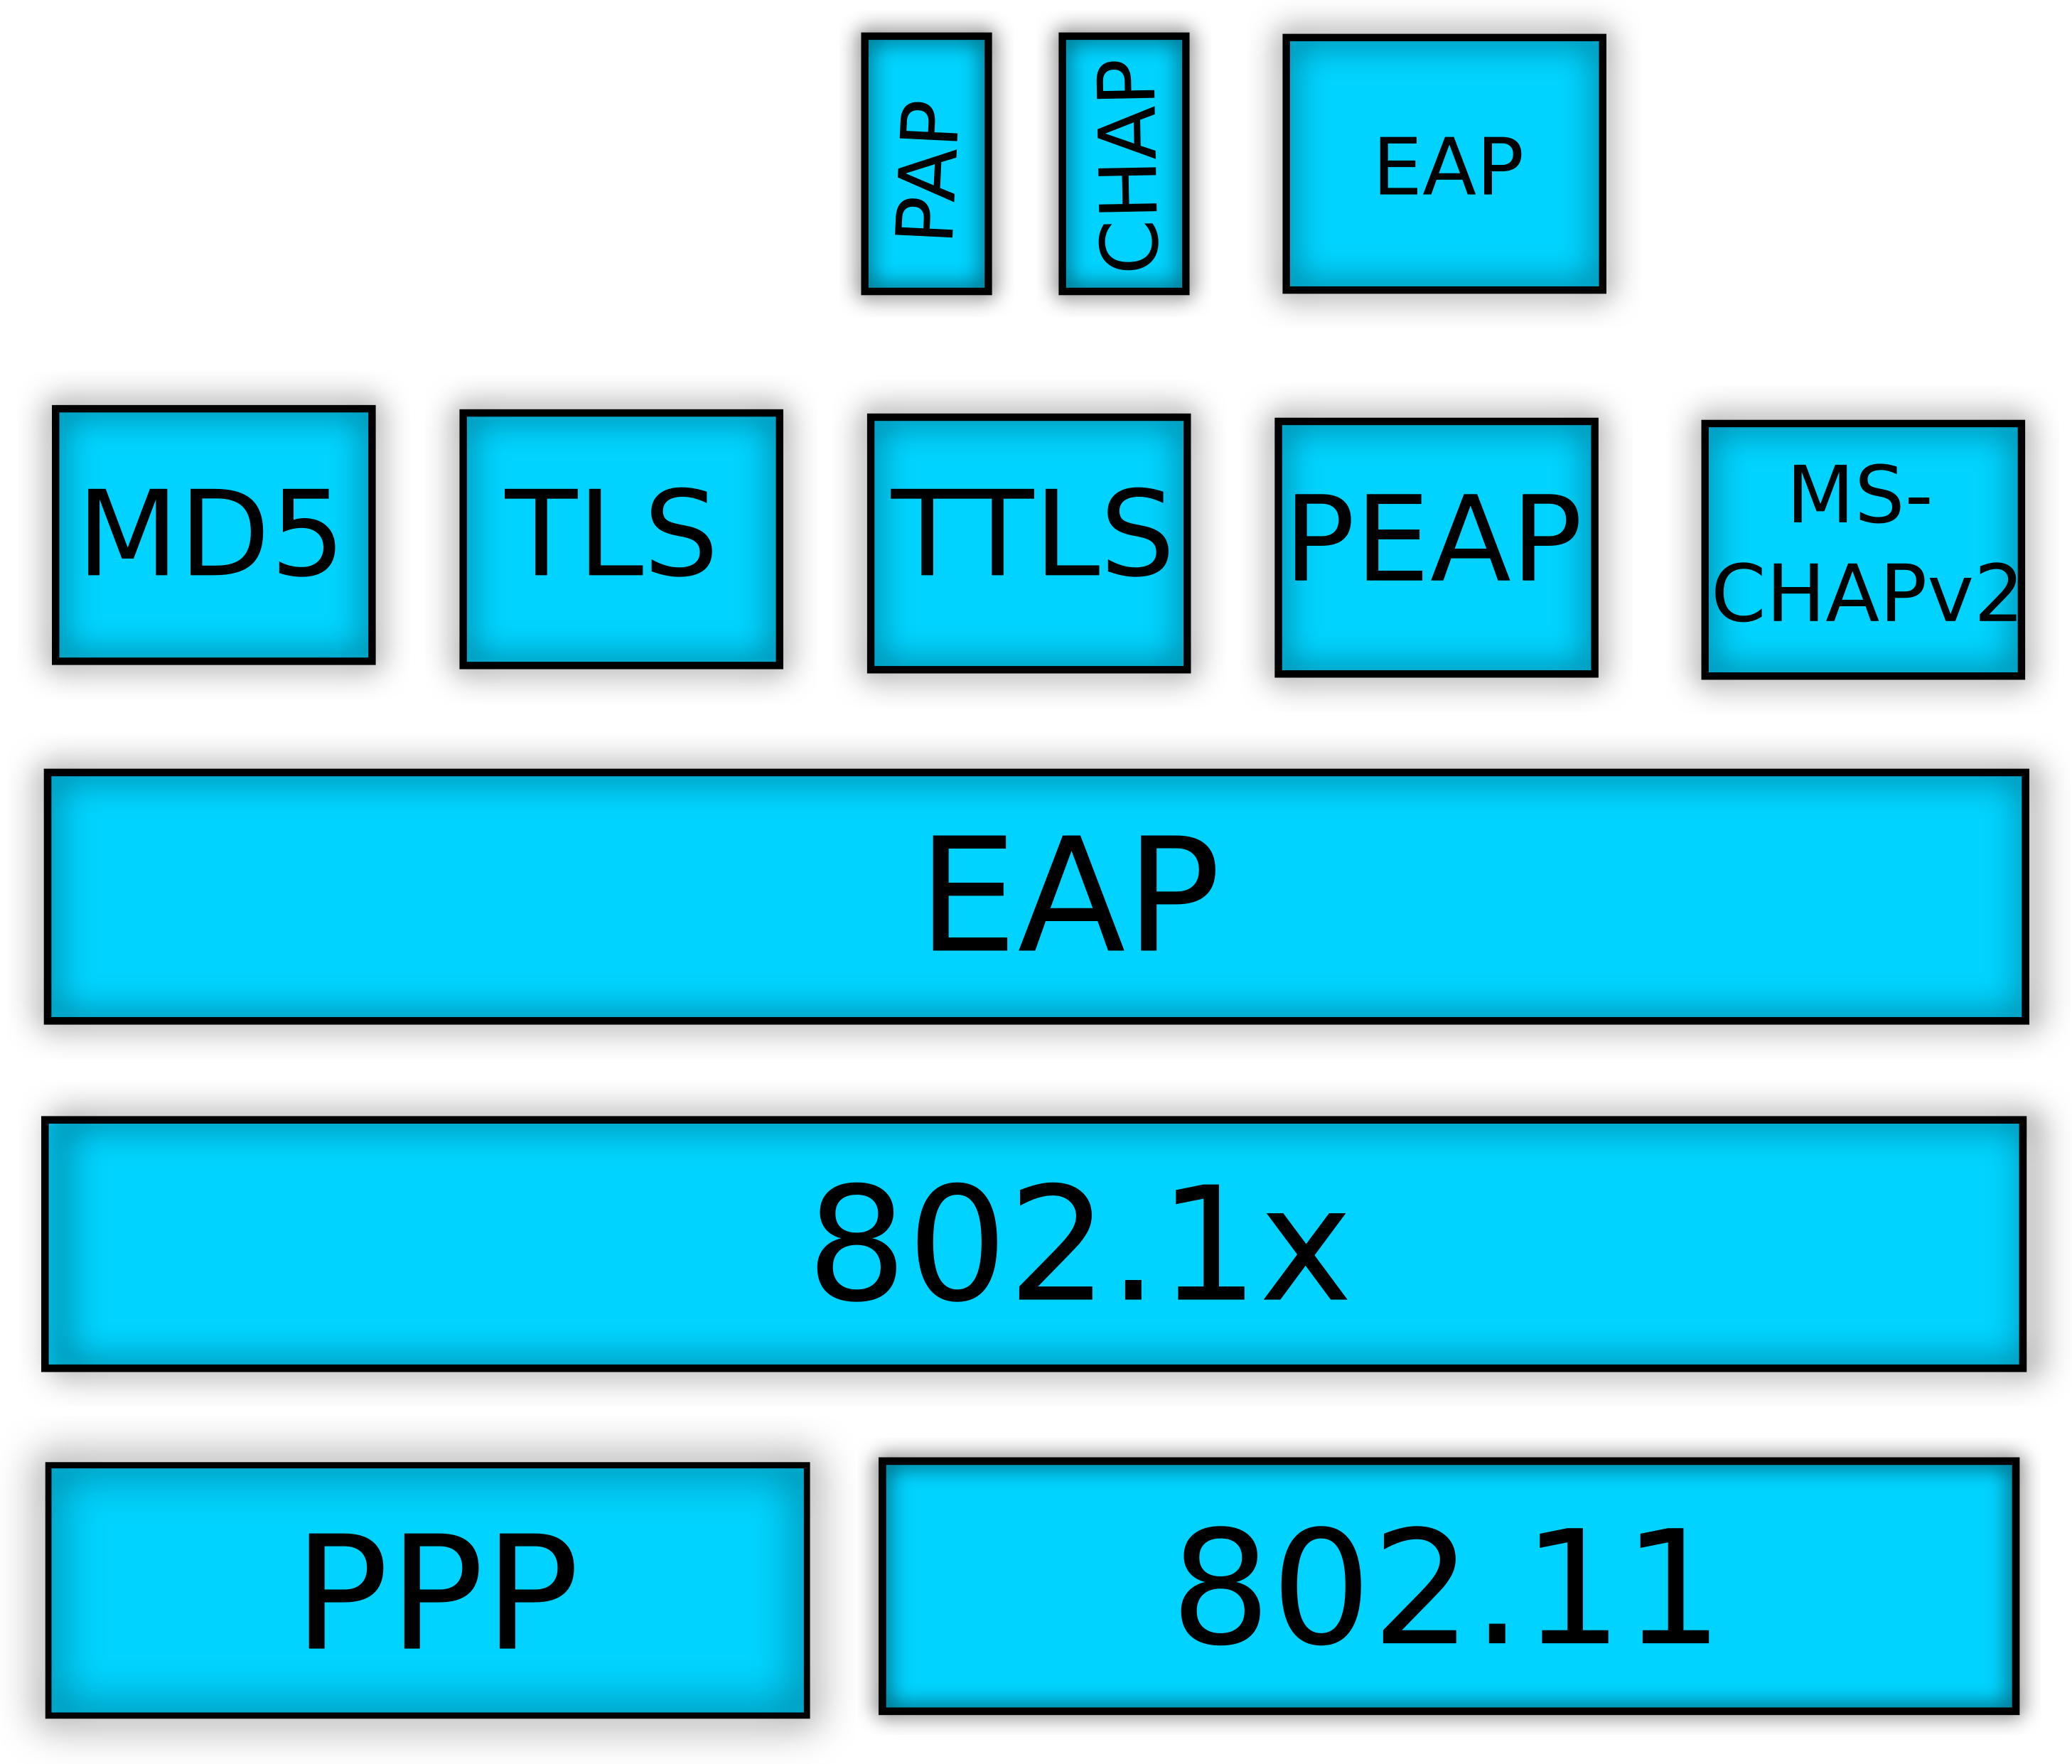
\includegraphics[width=0.48\textwidth]{graphics/EAP_packet_structure.png}
	\caption{EAP packet structure\protect\footnotemark}
	\label{fig:eap}
\end{figure}

\footnotetext{Adapted from \url{https://www.ixbt.com/comm/prac-wpa-eap.shtml}}

\subsection{IEEE 802.1x}

IEEE 802.1x is a port-based network access control and provides authentication mechanism to devices wishing to attach to LAN or WLAN~\cite{}. Overall, IEEE 802.1x defines 
encapsulation of the EAP over IEEE 802.3 and 802.11 networks, which is known as EAP over LAN or simple EAPOL. According to this standard whenever IEEE 802.3 Ethernet, or in case of wireless network IEEE 802.11, user attaches to network, the port remains closed and the network switch or wireless access point will forward only packets between the end-user and AAA server such as RADIUS. When wired switch or wireless access point receives EAPOL frame it will wrap those inside RADIUS packets and send to the RADIUS server. On the other hand, when RADIUS responds, the EAP packets will be stripped from RADIUS packet and forwarded to an end-user as EAPOL frame. The IEEE 802.1x port will be trusted, or authorized and, thus, all traffic will be allowed only, after reception of Access Accept message from the RADIUS server.

\subsection{RADIUS protocol} 

Remote Authentication Dial-In User Service (RADIUS) is a networking protocol, 
operating over User Datagram Protocol (UDP) on port 1812 (accounting is 
performed on 1813 UDP port). The protocol provides centralized authentication, 
authorization, and accounting (AAA or Triple A) management for users who 
connect to and use network services.

RADIUS was designed to serve the purpose of allowing a NAS to forward a 
dial-up user’s request and its credentials to a backend server. RADIUS 
was originally designed to accommodate PAP (password authentication protocol) and 
CHAP (challenge handshake authentication protocol). The specification of 
RADIUS protocol consists of several RFCs: RFC 2058, RFC 2138, RFC 2865 and RFC 2866. 

In RADIUS typically exist three parties who participate in 
authentication, authorization and accounting: an end user, wishing to gain access to a network,
Network Access Server (NAS), which usually acts as RADIUS client and Access Server (AS), which checks
credentials, makes admission decisions and can also optionally return configuration information
to a client.

RADIUS message set is rather simple and consist only of eight messages, of which only 
first four are specified in the base specification~\cite{AAA}. The six most commonly 
used messages are: 

\begin{itemize}
\item \textbf{Access request}. This message is generated by the NAS towards the RADIUS server
to forward the request from or on behalf of a user.	
\item \textbf{Access challenge}. This message is sent by RADIUS server towards the client to question 
the user about the knowledge of a secret.
\item \textbf{Access accept}. This message is sent by the RADIUS server to NAS to indicate the successful
completion of request. 
\item \textbf{Access reject}. This message is sent by the RADIUS server to NAS to indicate the 
rejection of a request.
\item \textbf{Accounting request}. This message is sent from NAS to RADIUS server to convey the 
accounting information.
\item \textbf{Accounting response}. This message is sent by the RADIUS server to the NAS to acknowledge 
that the accounting information sent previously by the client has been received. The message also 
indicates the result of the performed accounting function by the server.
\end{itemize}

In Figure~\ref{fig:radius_packet} we show the basic RADIUS packet structure. The first byte is the message type 
code. Next byte is identifier, which is used for matching requests with responses. Next two 
bytes used to store the length of the RADIUS packet including the code, identifier, length, 
authenticator and optional attributes. Authenticator field is 16 bytes 
long and is used for security purposes. The authenticator field (in request packets) is merely a random 
string of 16 bytes and is used to authenticate replies from the RADIUS server. In that manner, in 
response packets authenticator field contains MD5 hash over code field, identifier, length, 
request authenticator field from the access-request packet, and response attributes, 
followed by the shared secret. We should note that passwords transmitted in RADIUS packets
are also secured with so-called password hiding mechanism, which is a keyed version of MD5 hash.
Shared secret followed by the request authenticator field is put through a one-way
MD5 hash to create a 16 bytes digest value which is XORed with the password entered 
by the user, and the XORed result is placed in the user-password attribute in the 
access-request packet (the reverse operation is trivial if a party known the shared secret). 
More detailed definition of RADIUS packet formats can be found in RFC 2865.

\eat{Here a shared secret (between RADIUS client and server) is used to prevent eavesdroppers from modifying the packets in flight. Since MD5 is not secure, additional protection, such as IPSec tunnels, can be used to further protect RADIUS traffic between NAS device and access server.}

The attribute-value pairs (AVP) carry data in both requests and responses. The AVP consists of the 
attribute type, attribute length and attribute value. Almost every hardware manufacturer creates 
its own list of attributes. In our Enterprise WLAN setup, among many other attributes, we will use Mikrotik-Total-Limit and Mikrotik-Rate-Limit attributes, so that the NAS can rate-limit the 
connections as well as limit the amount of traffic received and transmitted.

\begin{figure}[!h]
	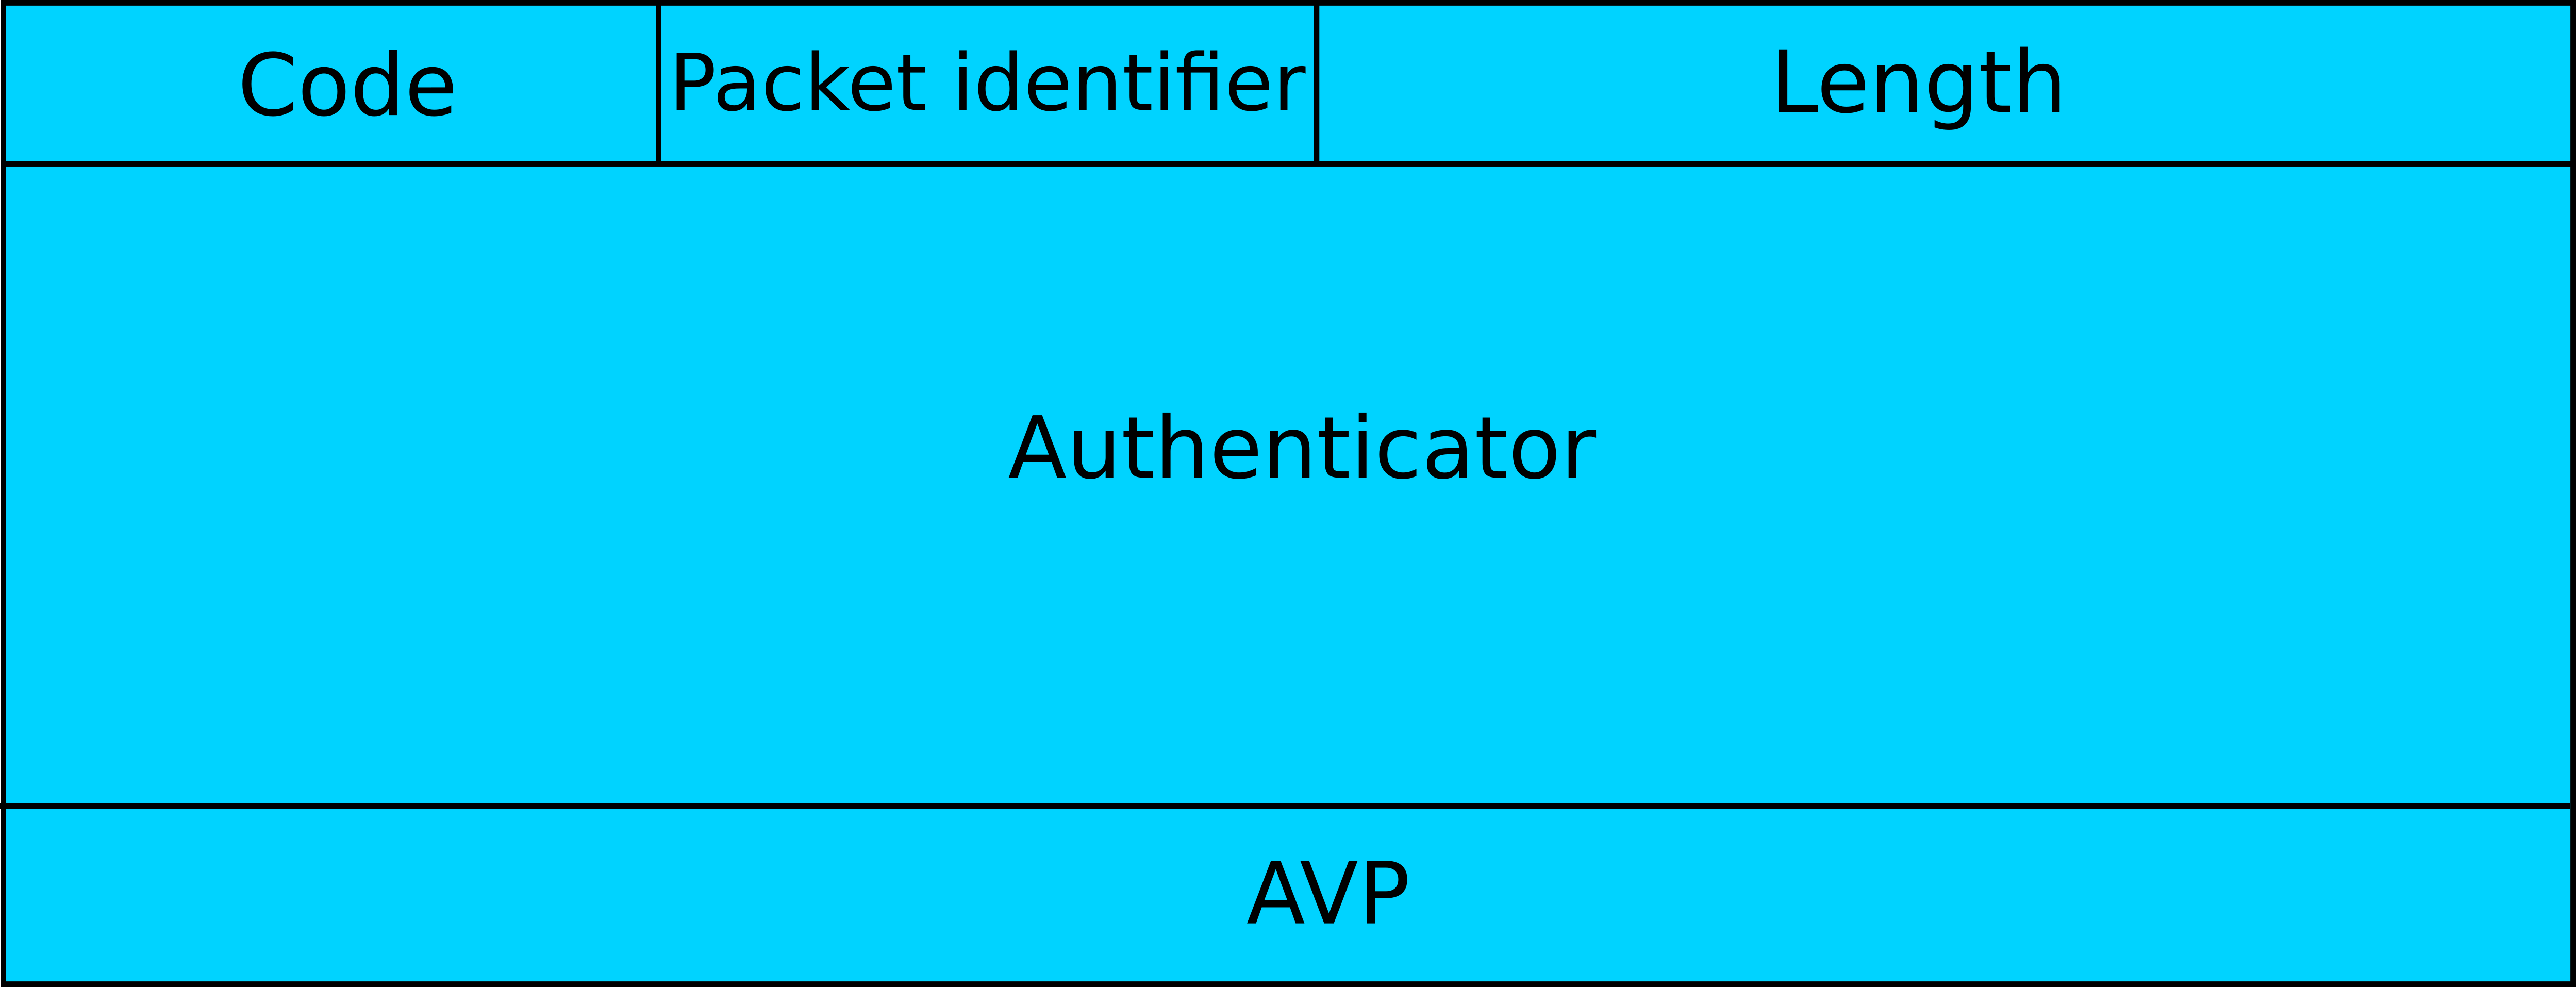
\includegraphics[width=0.48\textwidth]{graphics/radius_packet.png}
	\caption{Radius packet structure}
	\label{fig:radius_packet}
\end{figure}

\eat{
To understand how the authentication works in RADIUS, in the current paragraph 
we use CHAP authentication as an example. In what follows we will describe the operation 
of CHAP. Accordingly, at first, a user, which is configured to authenticate 
through CHAP, requests NAS to connect to network. At this point the user sends its identity 
to NAS. In response, NAS generates $16$ bytes random number and sends it back to the user 
though CHAP challenge message. The user responds to the challenge with the CHAP ID, 
CHAP username, and response to challenge which is computed as $MD5(ID, secret, challenge)$. 
NAS then creates an Access Request RADIUS message, which contains 
username, challenge, ID, and computed response to challenge in form of attributes. 
The RADIUS server, upon receiving the Access Requests, looks up password and computes $MD5(ID, 
secret, challenge)$. If the value found in Access Request matches the value computed by the 
server, the RADIUS server sends Access Accept message, otherwise an Access Reject message is 
sent back to the NAS.
}

\begin{figure}[!h]
	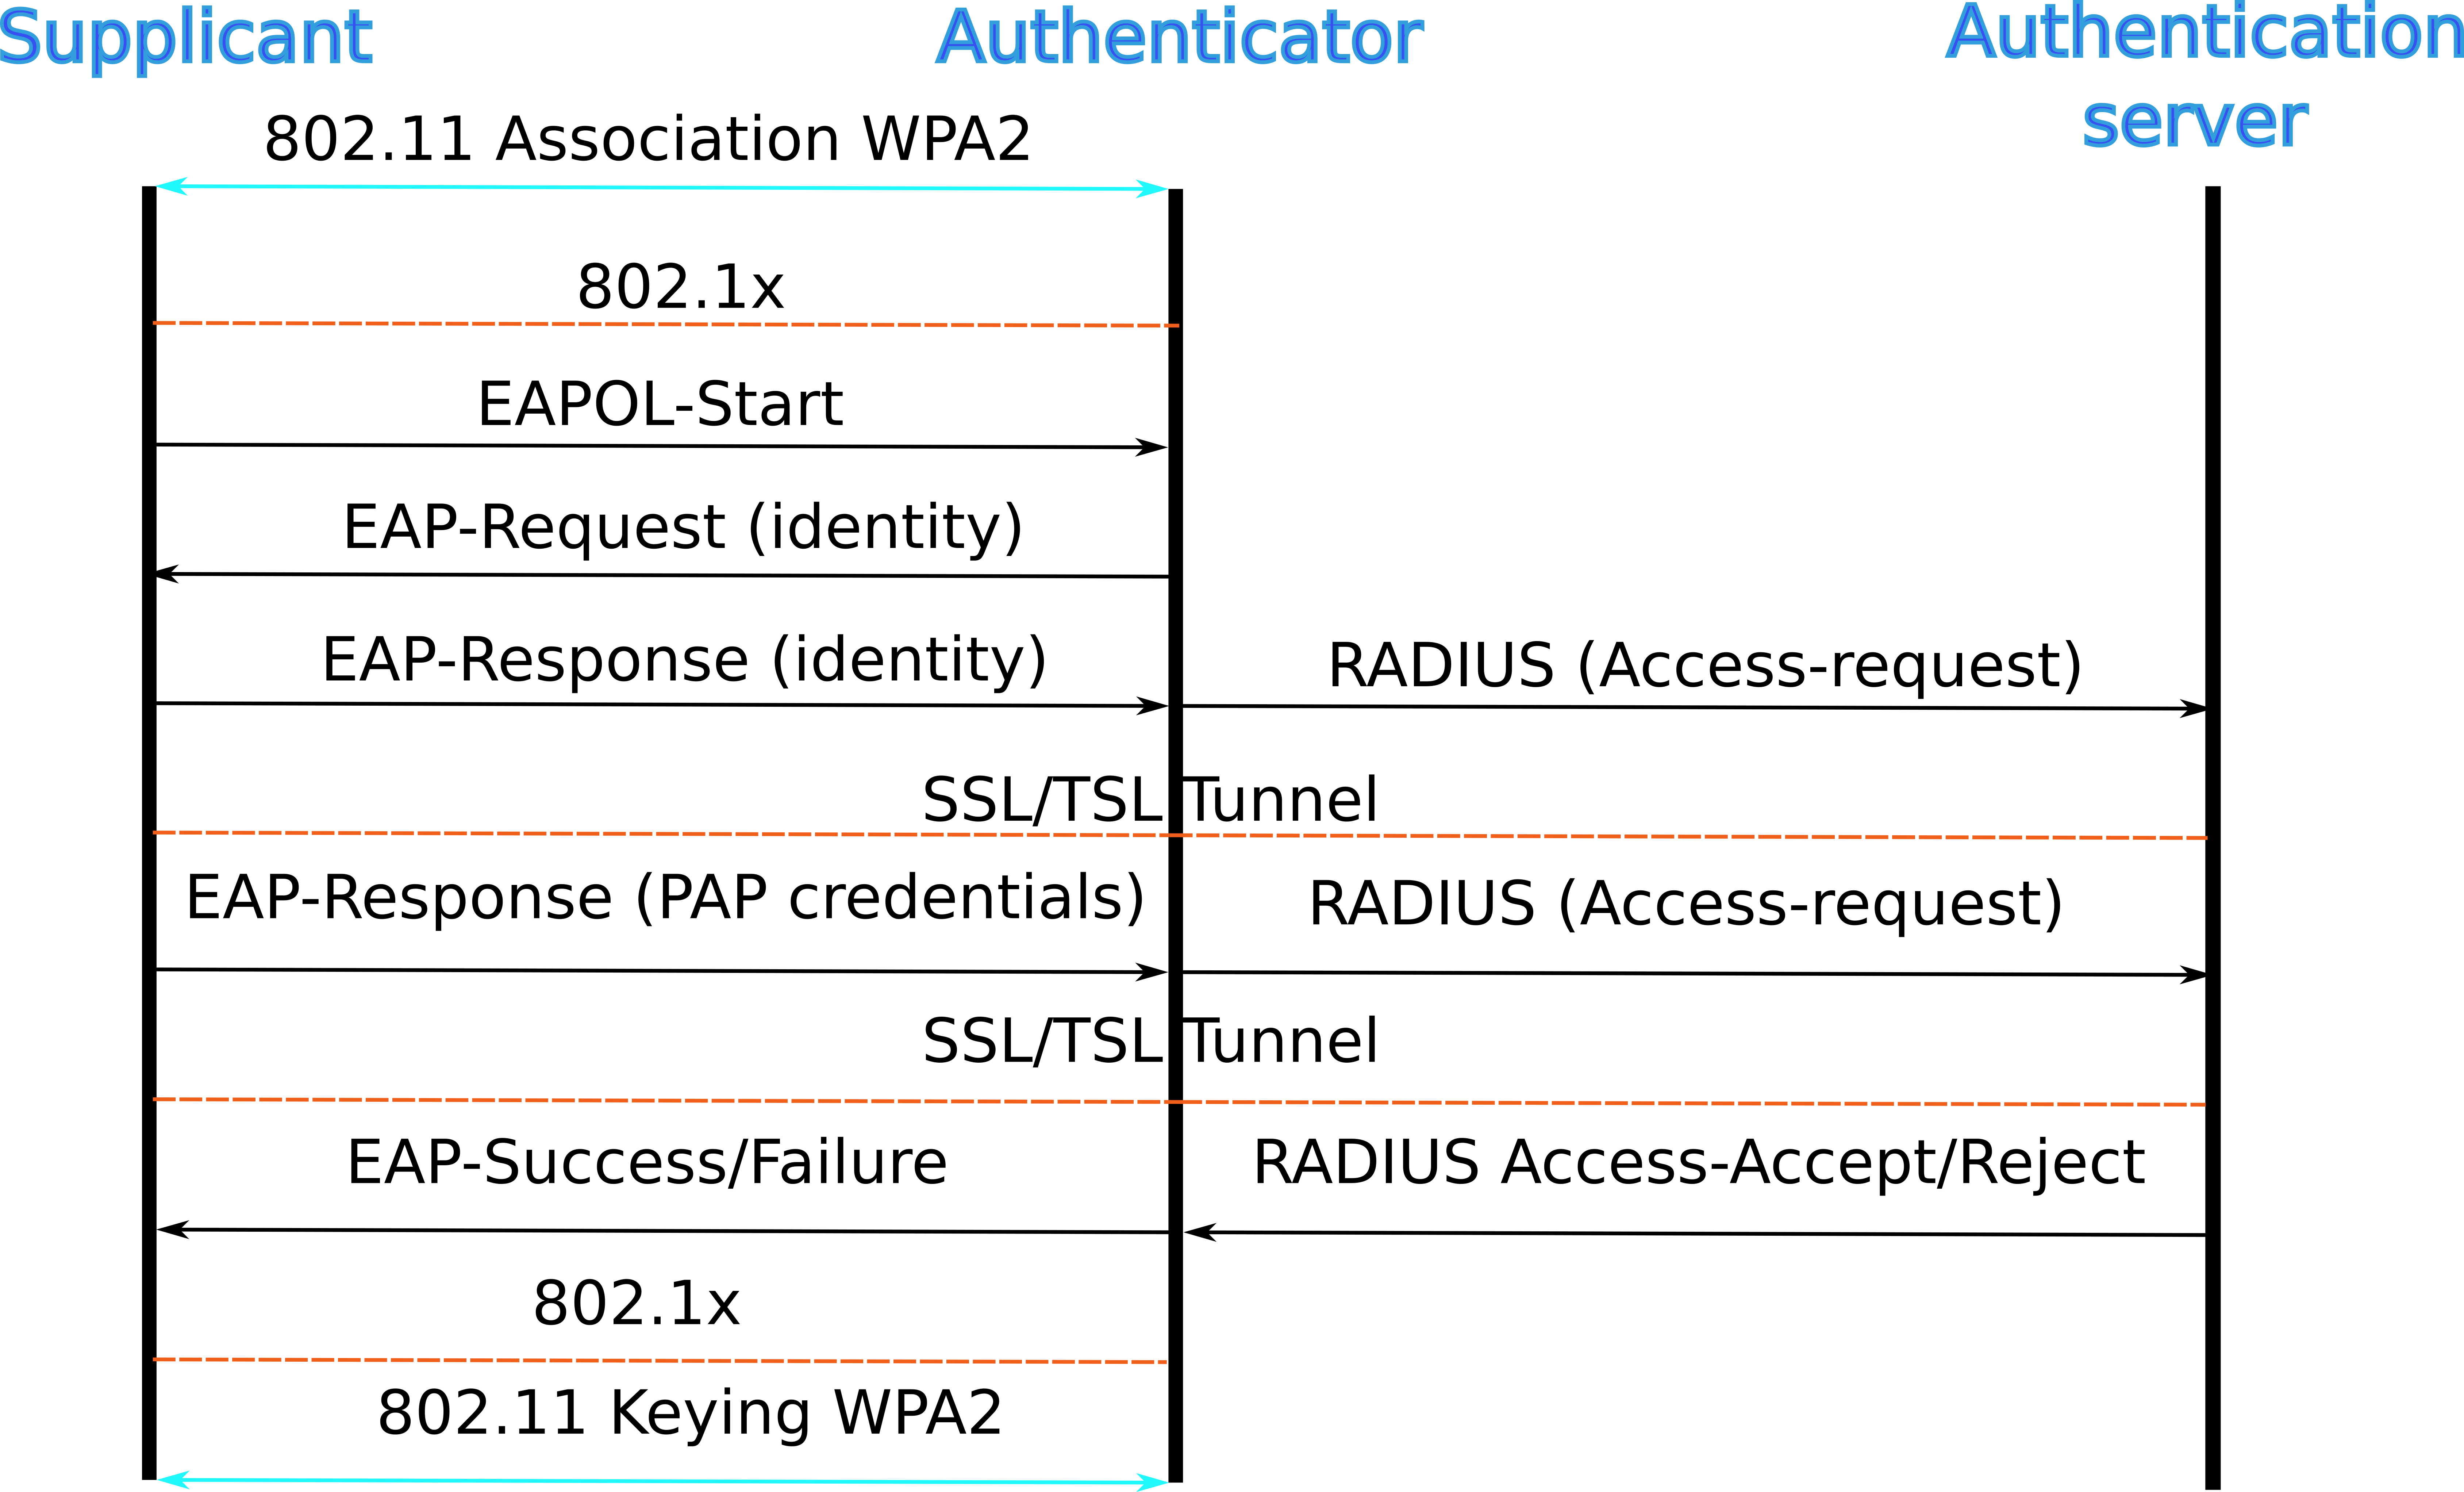
\includegraphics[width=0.48\textwidth]{graphics/EAP-TTLS.png}
	\caption{EAP usage in 802.11 WPA2 Enterprise setting\protect\footnotemark}
	\label{fig:eap}
\end{figure}


In addition to PAP and CHAP, RADIUS can also be used to carry 
EAP messages. In Figure~\cite{fig:eap-ttls} we demonstrate the interaction of 
end-user with the NAS and AS over EAP-TTLS. \eat{To understand the protocol better we have 
used the capture of EAP-TLS traffic and analyzed it using Wireshark~\cite{wireshark} software. 
According to the data, the protocol executes as follows. It starts with the wireless station
association. After a successful association, the access station sends 
EAPOL-Start packet. The Access Point responds with the EAP-Request (code \texttt{0x1}),
At this time, the end-user device answers with the EAP-Response (code \texttt{0x2}) with attribute 
type - \textit{Identity} (type \texttt{0x1}) and the value of actual identity. The server 
responds with the EAP-Request (code \texttt{0x1}) and type TLS EAP (type \texttt{0x13}).
The end-user responds with EAP-Response (code \texttt{0x2}) and TLS data containing 
Client-Hello message. After this, server responds with EAP-Request packet containing 
TLS Server Hello, Certificate, Server Key Exchange (Elliptic Curve Diffie-Hellman Server parameters) 
and Multiple Handshake Messages (Certificate Request and Server Hello Done). 
Next follows EAP-Response packet containing Client Certificate, Client Key Exchange 
(Elliptic Curve Diffie-Hellman Client parameters), Certificate Verify (proof that the client 
knows the private key) and Encrypted Handshake Message (to verify that the client correctly 
derived secret key). The server sends the Encrypted Handshake Message (as a proof that the server
derived correctly the secret key) and Change Cipher Spec message. Finally, the client sends 
EAP-Response for which the server sends EAP-Success (code \texttt{0x3}). If any of these steps will fail
the server will send EAP-Failure. Since RADIUS delivers Pairwise Master Key to NAS, 
after EAP-Success packet follows $4$-way handshake, which allows NAS 
(authenticator in EAP terminology) and end-user (supplicant in EAP terminology) to derive  
session keys.}

\footnotetext{Adapted from \url{https://www.eduroam.us/docs/tech_overview}}

\subsection{Wireless encryption algorithms}

In this section we will discuss the solutions which allow users to send messages 
in an encrypted format over wireless links. More specifically, the focus will be 
on wireless IEEE 802.11 networks.

\textbf{WEP}, or Wired Equivalent Privacy, is an old standard which defines how 
the keying material is derived, what encryption and message authentication algorithms to 
be used. For encryption, RC4 stream cipher is being used, which is known to be 
insecure~\cite{}. For integrity checks this standard employs CRC-32 algorithm.

\textbf{WPA}

\textbf{WPA-2}

\textbf{WPA-2 Enterprise} uses EAP framework for authentication and key management. In essence,
WPA-2 Enterprise uses the same algorithms for encryption, authentication and key management as 
WPA-2. The major difference is how the master secrets are derived: In WPA-2 Enterprise wireless 
station and authentication server use TLS protocol to negotiate master secret, later on the
authentication server delivers the keying material to access point using RADIUS protocol.

%\subsection{EAP-TTLS}

